\mychapter{1}{Appendix}
\section{Detailed BiCRS MACC Figures}
The following figures present detailed marginal removal cost curves of BECCS and Biochar, with breakdowns of the cost components as well as with and without leakage, transport and storage costs, and co-revenues.
\begin{figure}[ht]
%\vspace*{-\baselineskip}
  \begin{center}
    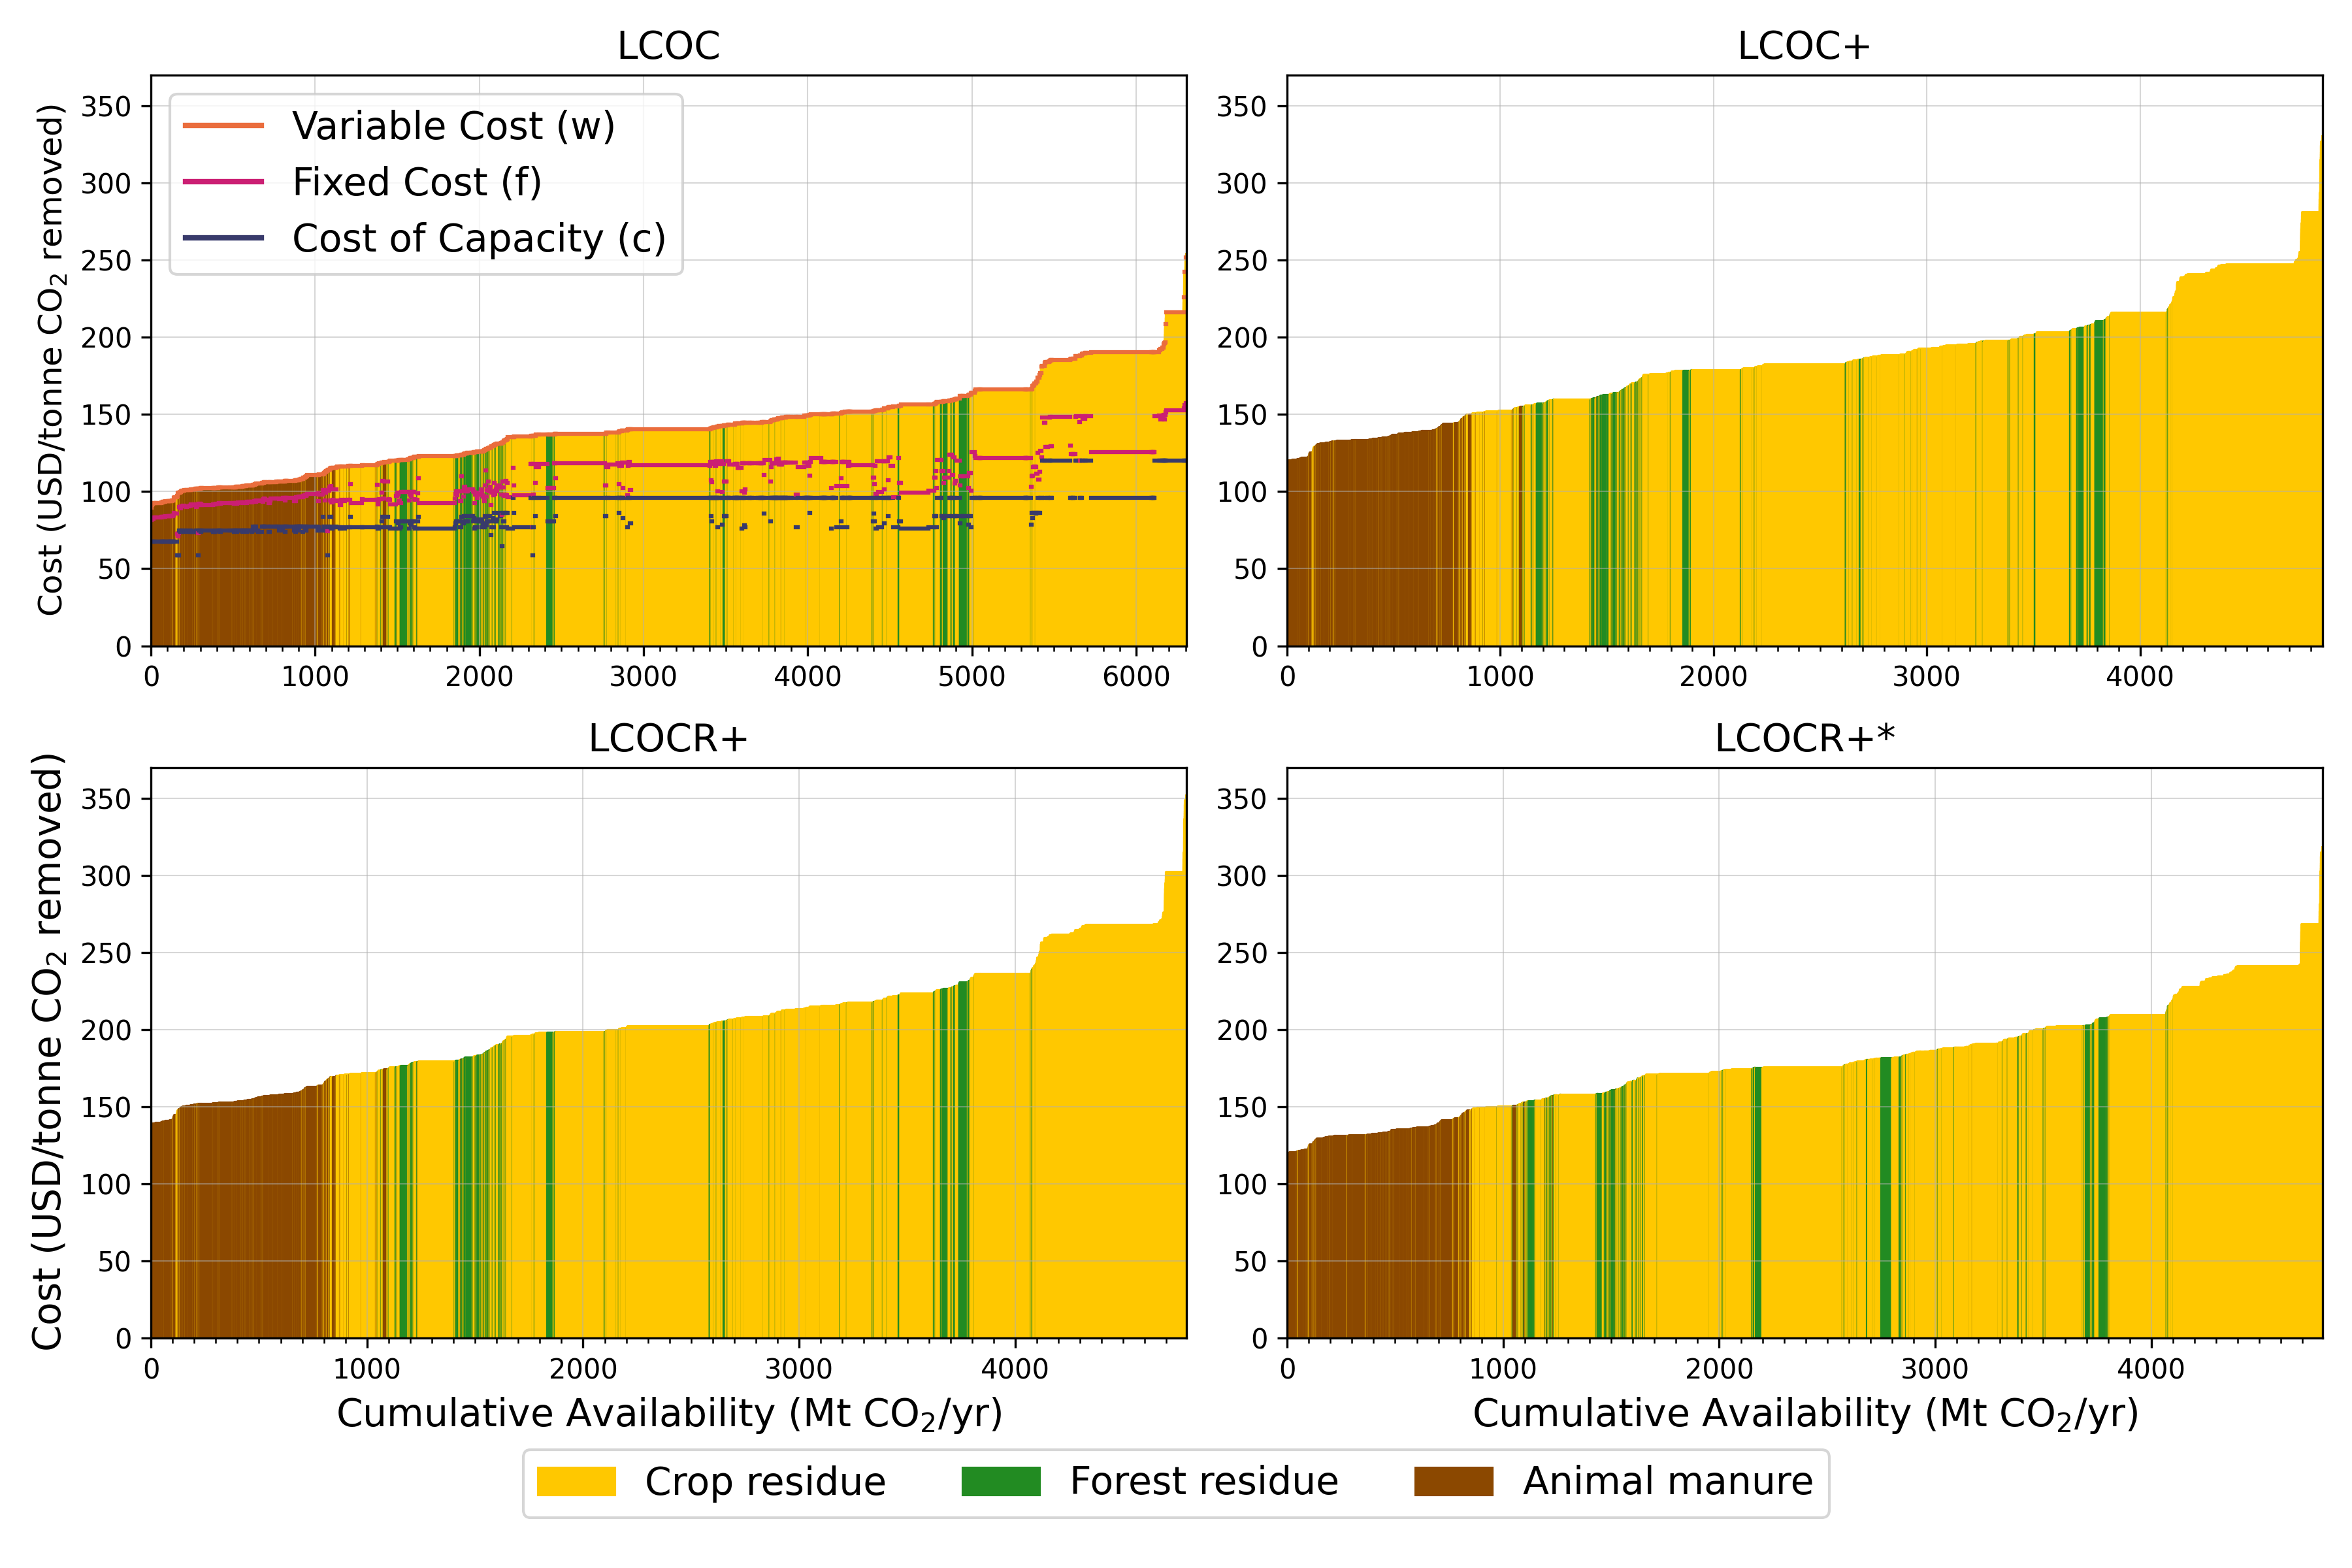
\includegraphics[width=0.87\linewidth]{figures/beccs_macc_chart.png}
    \caption{Detailed BECCS marginal removal cost curves}
    \label{fig:beccs_macc_chart}
  \end{center}
  \vspace{-2em}
\end{figure}

\begin{figure}[ht]
\vspace*{-\baselineskip}
  \begin{center}
    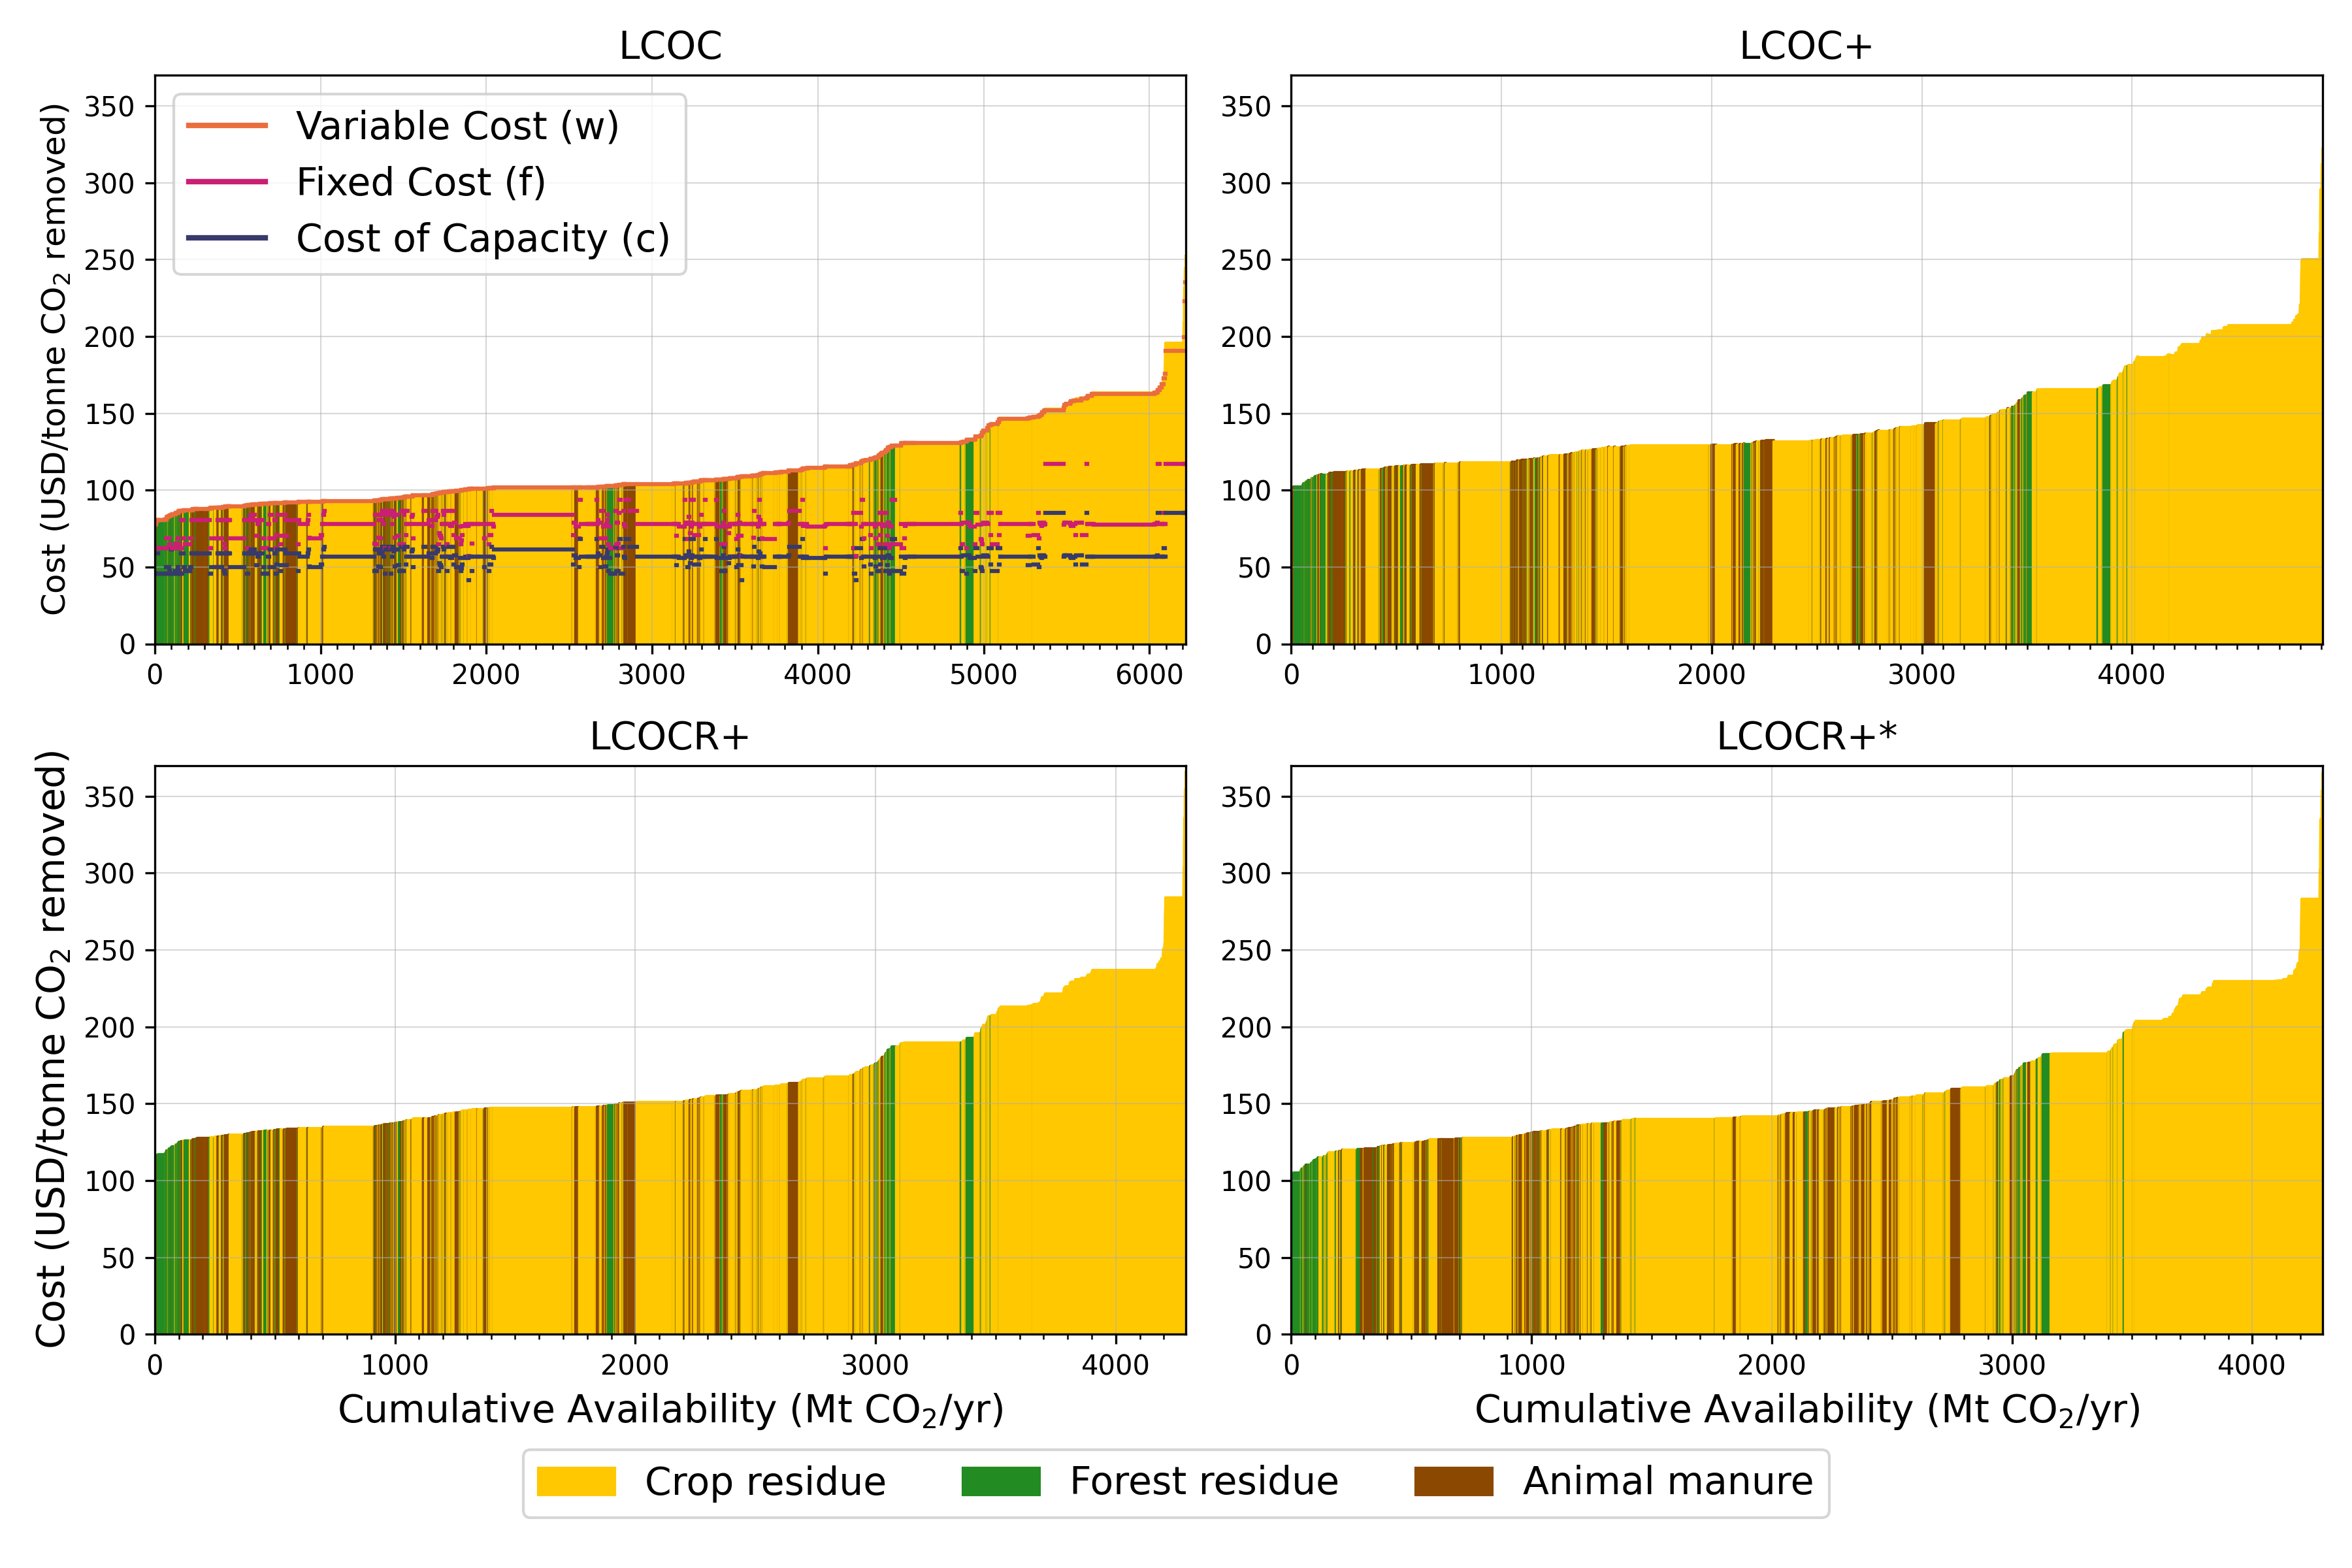
\includegraphics[width=0.87\linewidth]{figures/biochar_macc_chart.png}
    \caption{Detailed Biochar marginal removal cost curves}
    \label{fig:biochar_macc_chart}
  \end{center}
  \vspace{-2em}
\end{figure}

\newpage
\section{Derivation of Enhanced Weathering Formulas}
The original formula for the activation energy \(E_a\) from \textcite{wogelius_olivine_1992} used the Arrhenius relationship \parencite{arrhenius_uber_1889}, which describes the temperature dependence of chemical reaction rates, to calculate the activation energy of olivine rock:
\[
  E_a = 2.303 R         \cdot \frac{\log_{10}R_1-\log_{10}R_2}{\frac{1}{T_2}-\frac{1}{T_1}}.
\]
They computed the activation energy to be 79.5 kJ mol$^{-1}$ of olivine rock, based on their own experiments and previous literature. This formula was rearranged for the dissolution rate ($R_1$) at temperature $T_1$ (in Kelvin) based on known values for the activation energy and dissolution rate $R_2$ at temperature $T_2$, such that
\[
  \log_{10}R_1 = \frac{E_a}{2.303R}        \cdot\left(\frac{1}{T_2}-\frac{1}{T_1}\right) + \log_{10}R_2.
\]
This was then combined with the pH-based formula for the dissolution rate at 25 °C (= 262.15 K) defined by \textcite{hangx_coastal_2009}, so that
\[
  \log_{10}R_1 = 1.972R        \cdot\left(\frac{1}{262.15}-\frac{1}{K}\right) + \log_{10}R_{diss,25}(pH).
\]
With $R$ and $R_{{\text{diss}}, 25}(pH)$ plugged in, this resulted in the final equation for the dissolution rate based on temperature and pH value:
\begin{equation}
  \log_{10}{R_{\text{diss}}(pH, K)} = 16.4\left(\frac{1}{262.15}-\frac{1}{K}\right)-7.3656 - 0.297 \cdot pH.
\end{equation}

\hfill \break
\break
For the derivation of the average lifetime of a unit of rock, the integral of the shrinking core model designed by \textcite{hangx_coastal_2009} was used:
\[
  L = \int_0^{\infty}m(y)\,dy= \int_0^Y\left(1-\frac{y}{Y}\right)^3\,dy \quad\text{for } 0 \le y \le Y.
\]
By substituting \(u = \frac{y}{Y}\), this was re-writen to
\[
  L = \int_0^1(1-u)^3\,du \cdot Y = Y\int_0^1(1-u)^3\,du
\]
which was solved to yield
\[
  L = Y\left[-\frac{(1-u)^4}{4}\right]_{0}^{1} = Y\left[\left(-\frac{(1-1)^4}{4}\right)-\left(-\frac{(1-0)^4}{4}\right)\right] = \frac{Y}{4}.
\]

\newpage
\section{Sample ERW Mining Operation}
Tables A.1 and A.2 show the cost of the exemplary US-based ERW operation to remove 15 GtCO$_2$ per year. Note that the units are cost (USD) per tonne of rock material mined, processed, and applied, not in tonnes of CO$_2$ removed.
\begin{table}[h!]
\renewcommand{\arraystretch}{1.3}
\adjustbox{max width=\textwidth}{%
\begin{tabular}{llr}
\hline
\textbf{Parameter} & \textbf{Unit} & \textbf{Value} \\ \hline

\multicolumn{3}{l}{\textbf{Fixed cost}} \\ \hline
Total CapEx             & USD       & 100{,}500{,}000 \\
Annual maintenance      & \%        & 2.2 \\
Annual maintenance cost & USD       & 2{,}211{,}000 \\
\textbf{Total fixed cost} & \textbf{USD t$^{-1}$} & \textbf{0.147} \\ \hline

\multicolumn{3}{l}{\textbf{Variable cost}} \\ \hline

\multicolumn{3}{l}{\textit{Mining}} \\
Energy (drilling \& blasting) & kWh t$^{-1}$ & 5.23 \\
Energy cost                   & USD t$^{-1}$ & 0.23 \\
Labour required                       & hr t$^{-1}$   & 0.14 \\
Labour cost                   & USD t$^{-1}$ & 9.84 \\
\textit{Mining cost}          & \textit{USD t$^{-1}$} & \textit{10.07} \\

\multicolumn{3}{l}{\textit{Processing}} \\
Electric energy (grinding)    & kWh t$^{-1}$ & 150.35 \\
Energy cost                   & USD t$^{-1}$ & 6.62 \\
Labour required                       & hr t$^{-1}$   & 0.00 \\
Labour cost                   & USD t$^{-1}$ & 0.00 \\
\textit{Processing cost}      & \textit{USD t$^{-1}$} & \textit{6.62} \\

\multicolumn{3}{l}{\textit{Transport \& application}} \\
Transport distance (rail)     & km    & 1{,}000 \\
Transport distance (road)     & km    & 200 \\
Transport cost (rail)         & USD t$^{-1}$ & 8.08 \\
Transport cost (road)         & USD t$^{-1}$ & 6.18 \\
Spreading time                & hr ha$^{-1}$  & 0.5 \\
Spreading cost                & USD t$^{-1}$ & 2.58 \\
\textit{T\&A cost}     & \textit{USD t$^{-1}$} & \textit{16.83} \\

\textbf{Total variable cost}  & \textbf{USD t$^{-1}$} & \textbf{33.51} \\ \hline

\end{tabular}}
\caption{Cost structure of a sample US-based ERW operation (denoted in USD per tonne of olivine rock)}
\end{table}

\newpage

\begin{table}[h!]
\renewcommand{\arraystretch}{1.03}
\adjustbox{max width=\textwidth}{%
\begin{tabular}{llr}
\hline
\textbf{Parameter} & \textbf{Unit} & \textbf{Value} \\ \hline

\multicolumn{3}{l}{\textbf{General}} \\ \hline
Annual rock volume      & Mt       & 15 \\
Daily rock volume       & t        & 41{,}096 \\
Operating hours         & hr day$^{-1}$     & 12 \\
Machinery lifetime      & yr        & 20 \\ \hline

\multicolumn{3}{l}{\textbf{Mining}} \\ \hline
Drill rig capacity      & t day$^{-1}$     & 50{,}000 \\
Drill rigs required     & --        & 1 \\
Drill rig unit price    & USD       & 1{,}500{,}000 \\
Drill rig cost          & USD       & 1{,}500{,}000 \\

Loading time            & min       & 2 \\
Loader capacity         & t         & 70 \\
Loader capacity         & t hr$^{-1}$       & 2{,}100 \\
Loaders required        & --        & 2 \\
Loader unit price       & USD       & 2{,}000{,}000 \\
Loader cost             & USD       & 4{,}000{,}000 \\

Truck capacity          & t         & 100 \\
Truck avg. speed        & km h$^{-1}$      & 20 \\
Distance pit--grinder   & km        & 5 \\
Truck roundtrip time    & h         & 0.57 \\
Truck capacity          & t hr$^{-1}$       & 176 \\
Trucks required         & --        & 20 \\
Truck unit price        & USD       & 500{,}000 \\
Truck cost              & USD       & 10{,}000{,}000 \\

CapEx -- Mining         & USD       & 15{,}500{,}000 \\
\textbf{CapEx per tonne of rock}         & \textbf{USD t$^{-1}$}     & \textbf{0.10} \\ \hline

\multicolumn{3}{l}{\textbf{Processing}} \\ \hline
Crusher capacity        & t hr$^{-1}$       & 600 \\
Crushers required       & --        & 6 \\
Crusher unit price      & USD       & 2{,}500{,}000 \\
Crusher cost            & USD       & 15{,}000{,}000 \\

Primary Grinder capacity      & t hr$^{-1}$       & 100 \\
Primary Grinders required     & --        & 35 \\
Primary Grinder unit price    & USD       & 1{,}000{,}000 \\
Primary Grinder cost          & USD       & 35{,}000{,}000 \\

Secondary Grinder capacity      & t hr$^{-1}$       & 100 \\
Secondary Grinders required     & --        & 35 \\
Secondary Grinder unit price    & USD       & 1{,}000{,}000 \\
Secondary Grinder cost          & USD       & 35{,}000{,}000 \\

CapEx -- Processing     & USD       & 85{,}000{,}000 \\
\textbf{CapEx per tonne of rock}         & \textbf{USD t$^{-1}$}     & \textbf{0.53} \\ \hline

\multicolumn{3}{l}{\textbf{Total}} \\ \hline
Total CapEx             & USD       & 100{,}500{,}000 \\
\textbf{Total CapEx per tonne of rock}   & \textbf{USD t$^{-1}$}     & \textbf{0.63} \\ \hline

\end{tabular}}
\caption{Techno-economic parameters for a sample US-based ERW operation (denoted in USD per tonne of olivine rock)}
\end{table}

\clearpage
\section{Liquid DAC Learning Effects}
Figure A.3 shows the drop in capacity cost per unit of L-DAC. Compared to solid DAC, it starts significantly lower, but the drop in cost is less pronounced due to the lower assumed learning rates.
\begin{figure}[h!]
  \begin{center}
    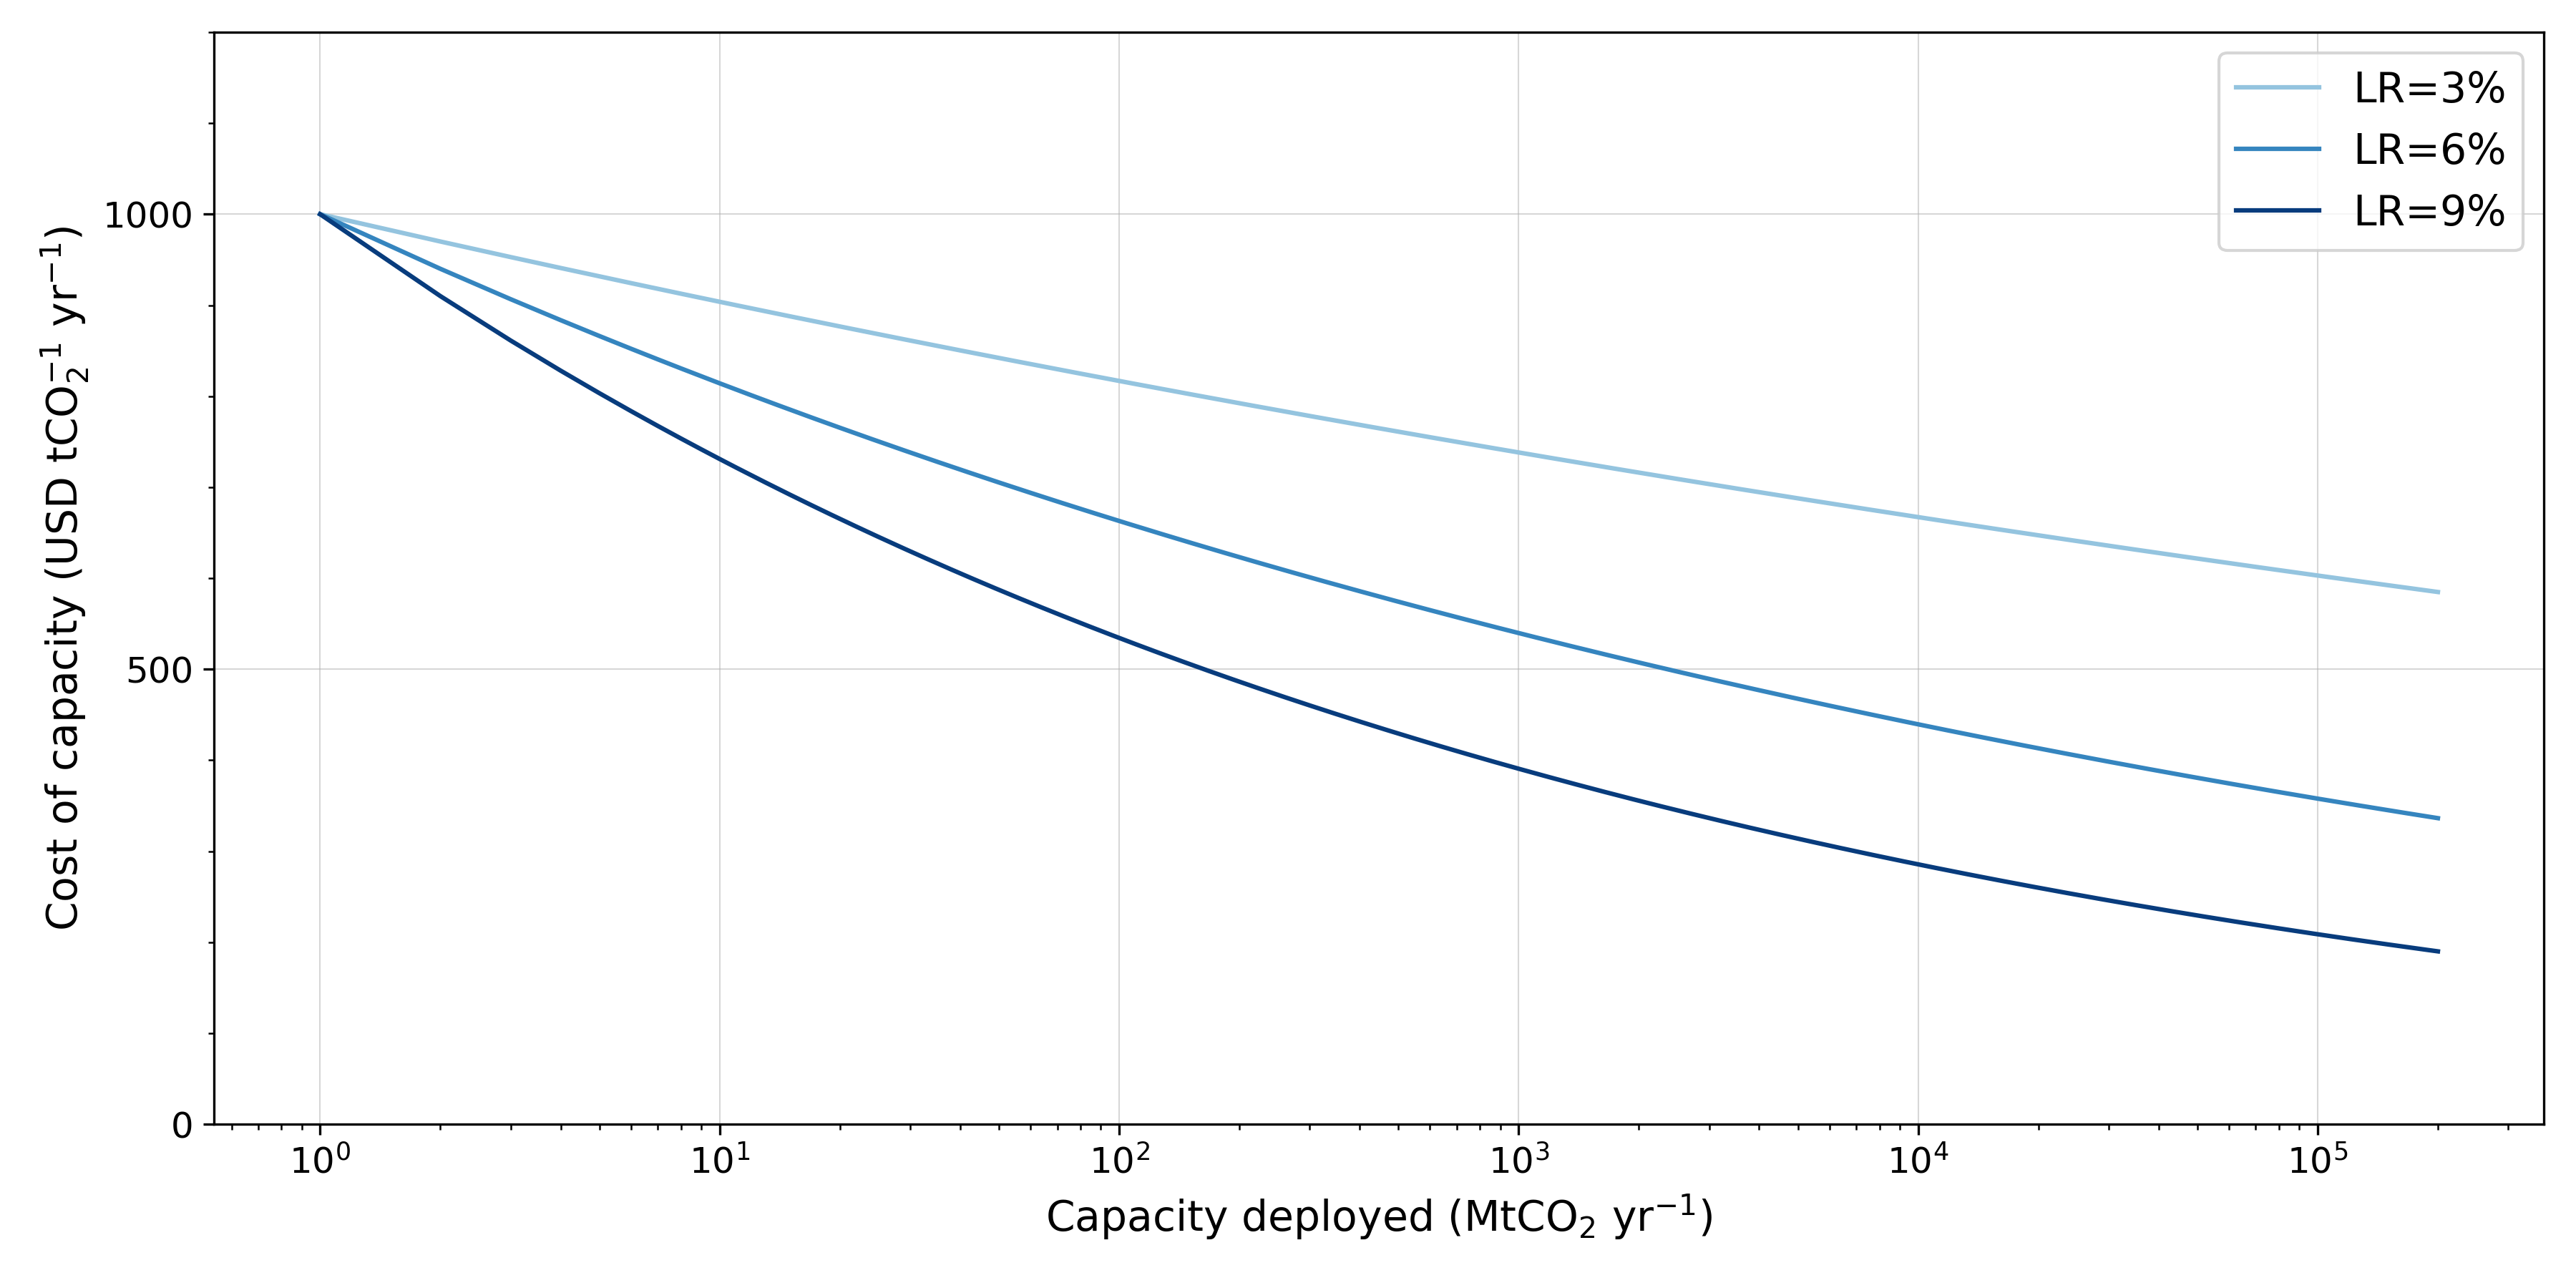
\includegraphics[width=1\linewidth]{figures/dac_learning_ldac.png}
    \caption{Exemplary liquid DAC CapEx learning curve}
    \label{fig:dac_capex_learning}
  \end{center}
\end{figure}

\clearpage
\section{Static Portfolio Removal Timelines}
Figures A.4 and A.5 show the deployment of the various NETs over time under the different time horizons considered in the static optimization model. Tables A.3 and A.4 show the corresponding total removals, total costs and average LCOCs.
\begin{figure}[h!]
  \begin{center}
    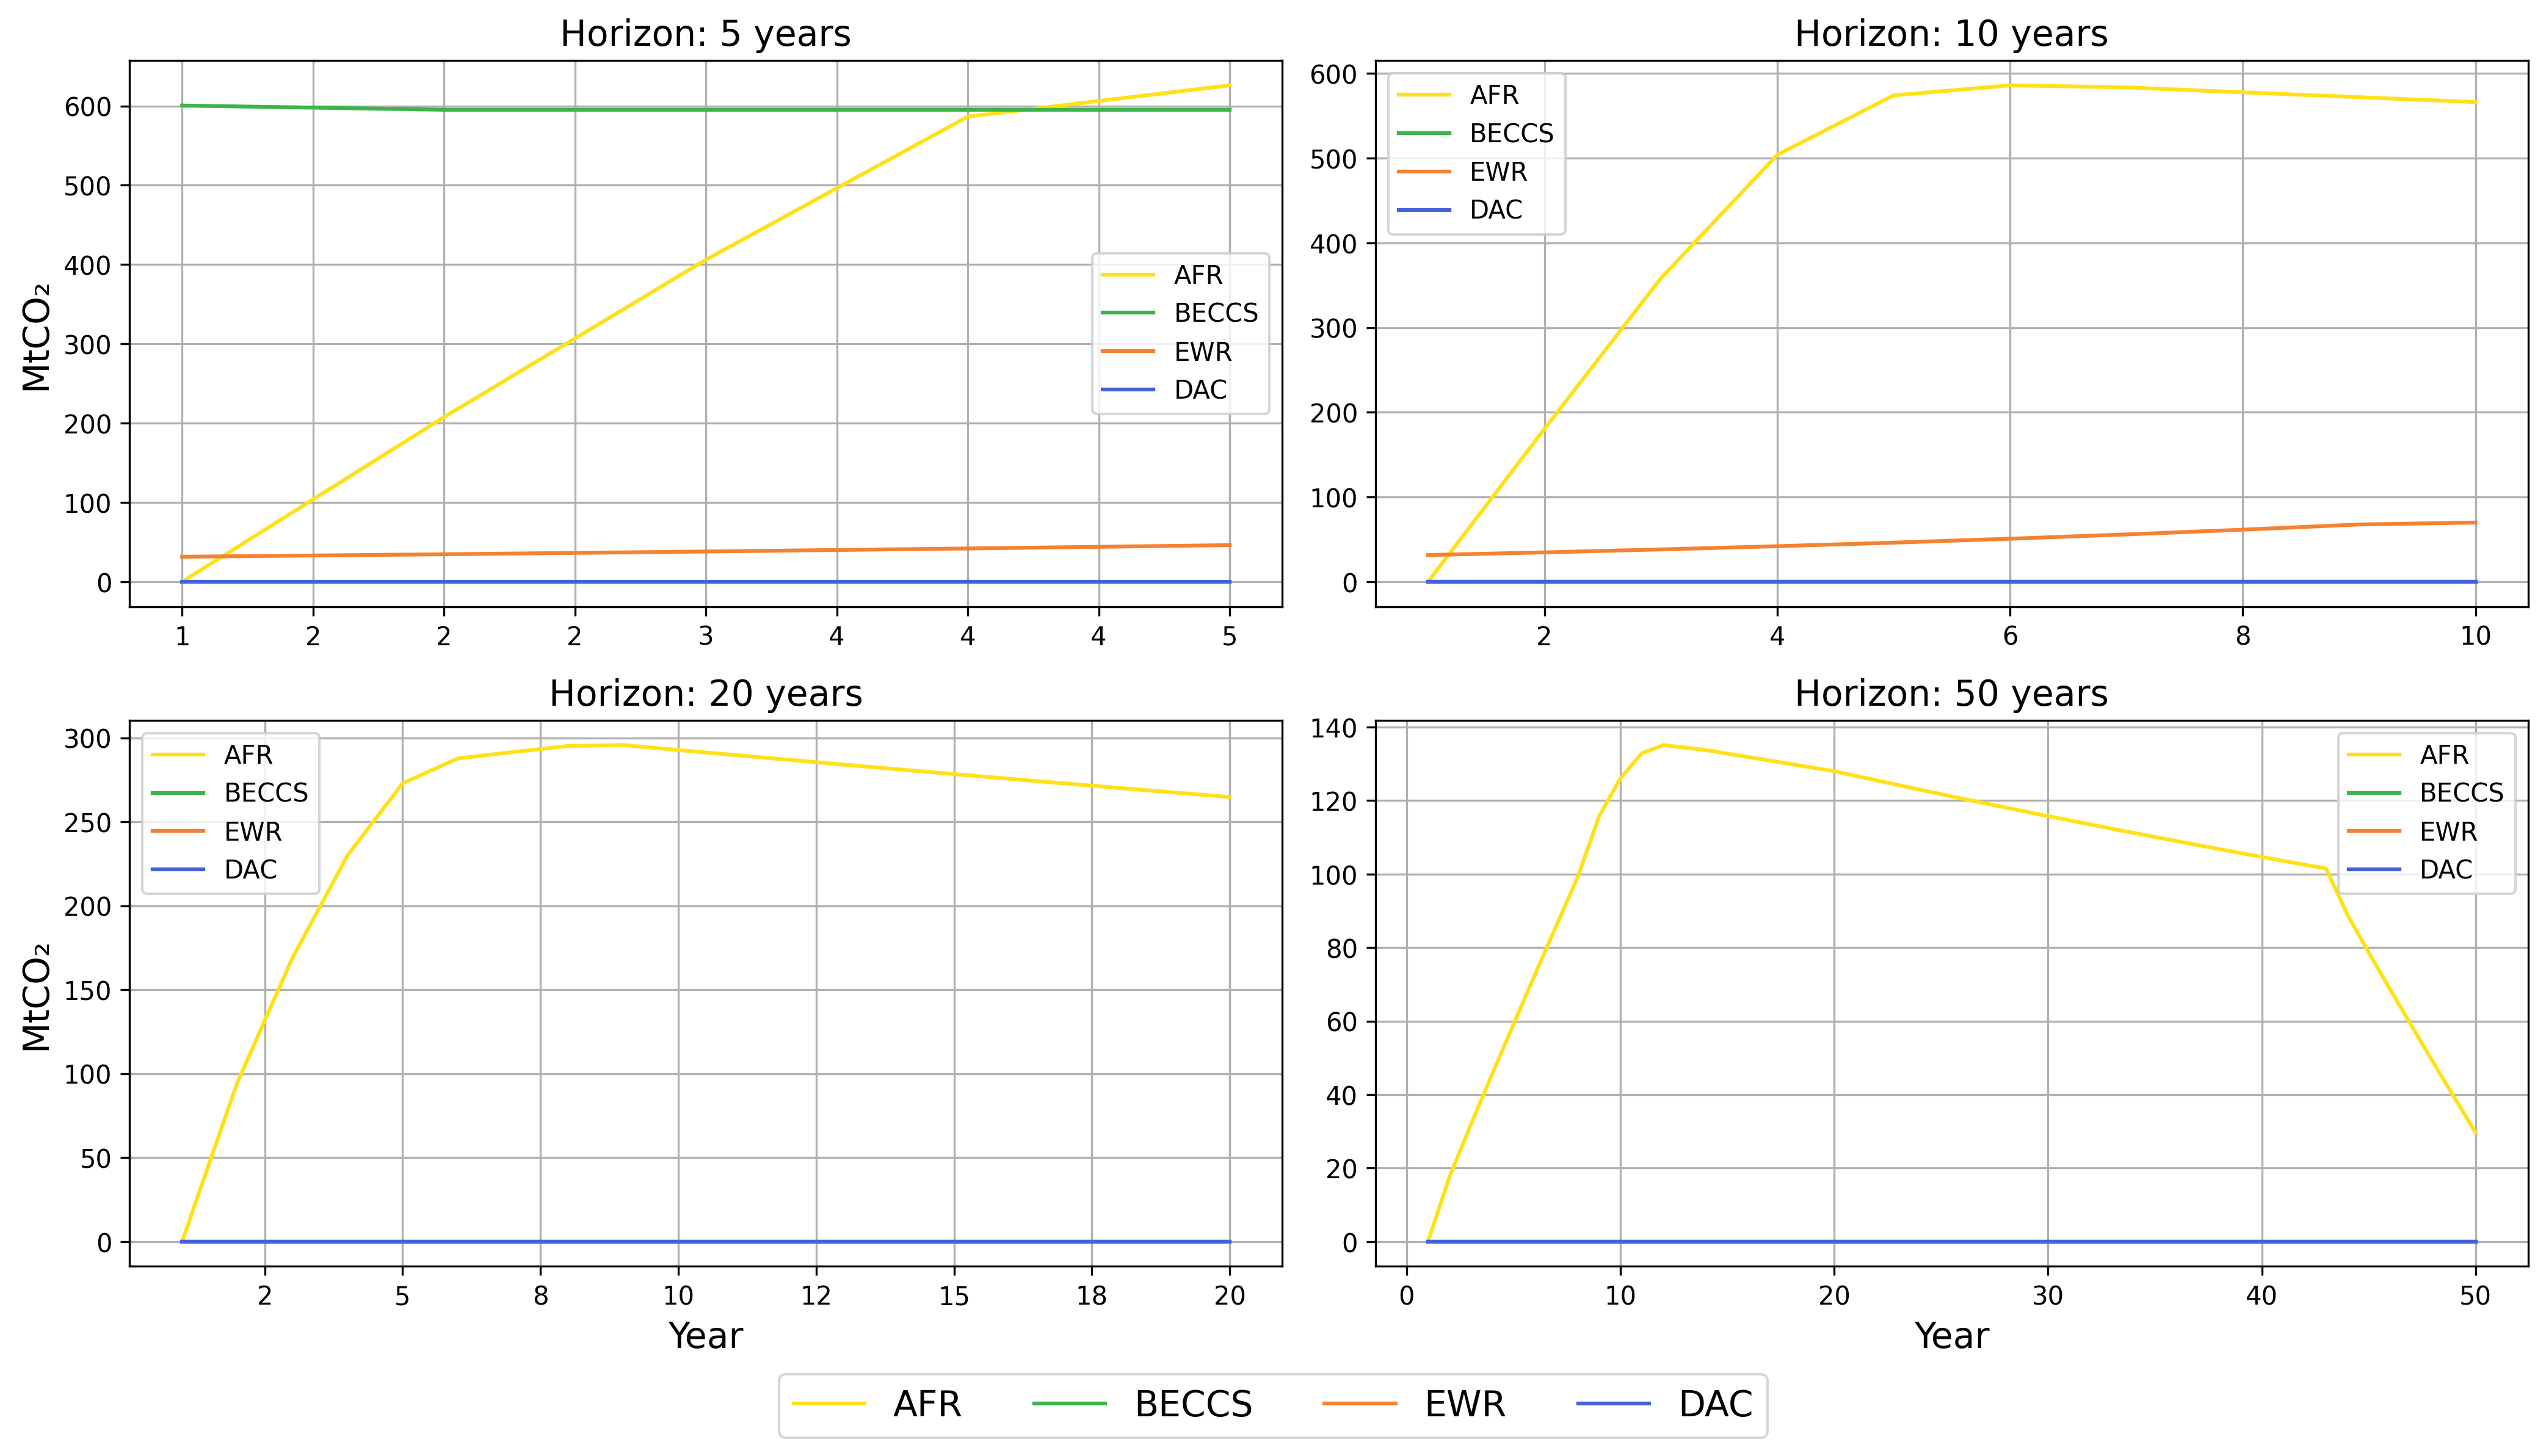
\includegraphics[width=\linewidth]{figures/overall_static_optimization_lines.png}
    \caption{Optimal static portfolio}
    \label{fig:overall_static_optimization_lines}
    \vspace*{-\baselineskip}
  \end{center}
\end{figure}

\begin{table}[h!]
\renewcommand{\arraystretch}{1.4}
\adjustbox{max width=\textwidth}{%
\begin{tabular}{llrrr}
\hline
\textbf{Horizon}          & \textbf{Technology} & \textbf{Total CDR (MtCO$_2$)} & \textbf{Total Cost (M USD)} & \textbf{Average LCOC (USD)} \\ \hline

\multirow{3}{*}{5 years}  
& A/R       & 1{,}915.8 & 114{,}830 & 59.94 \\
& ERW       & 34.9      & 890       & 25.52 \\
& BECCS     & 3{,}049.3 & 440{,}410 & 144.43 \\ \hline

\multirow{2}{*}{10 years} 
& A/R       & 4{,}920.6 & 96{,}557  & 19.62 \\
& ERW       & 79.4      & 2{,}026   & 25.52 \\ \hline

\multirow{1}{*}{20 years} 
& A/R       & 5{,}000.0 & 36{,}708  & 7.34 \\ \hline

\multirow{1}{*}{50 years} 
& A/R       & 5{,}000.0 & 13{,}172  & 2.63 \\ \hline

\end{tabular}}
\caption{Cost and deployment by CDR technology across time horizons}
\end{table}

\begin{figure}[h!]
  \begin{center}
    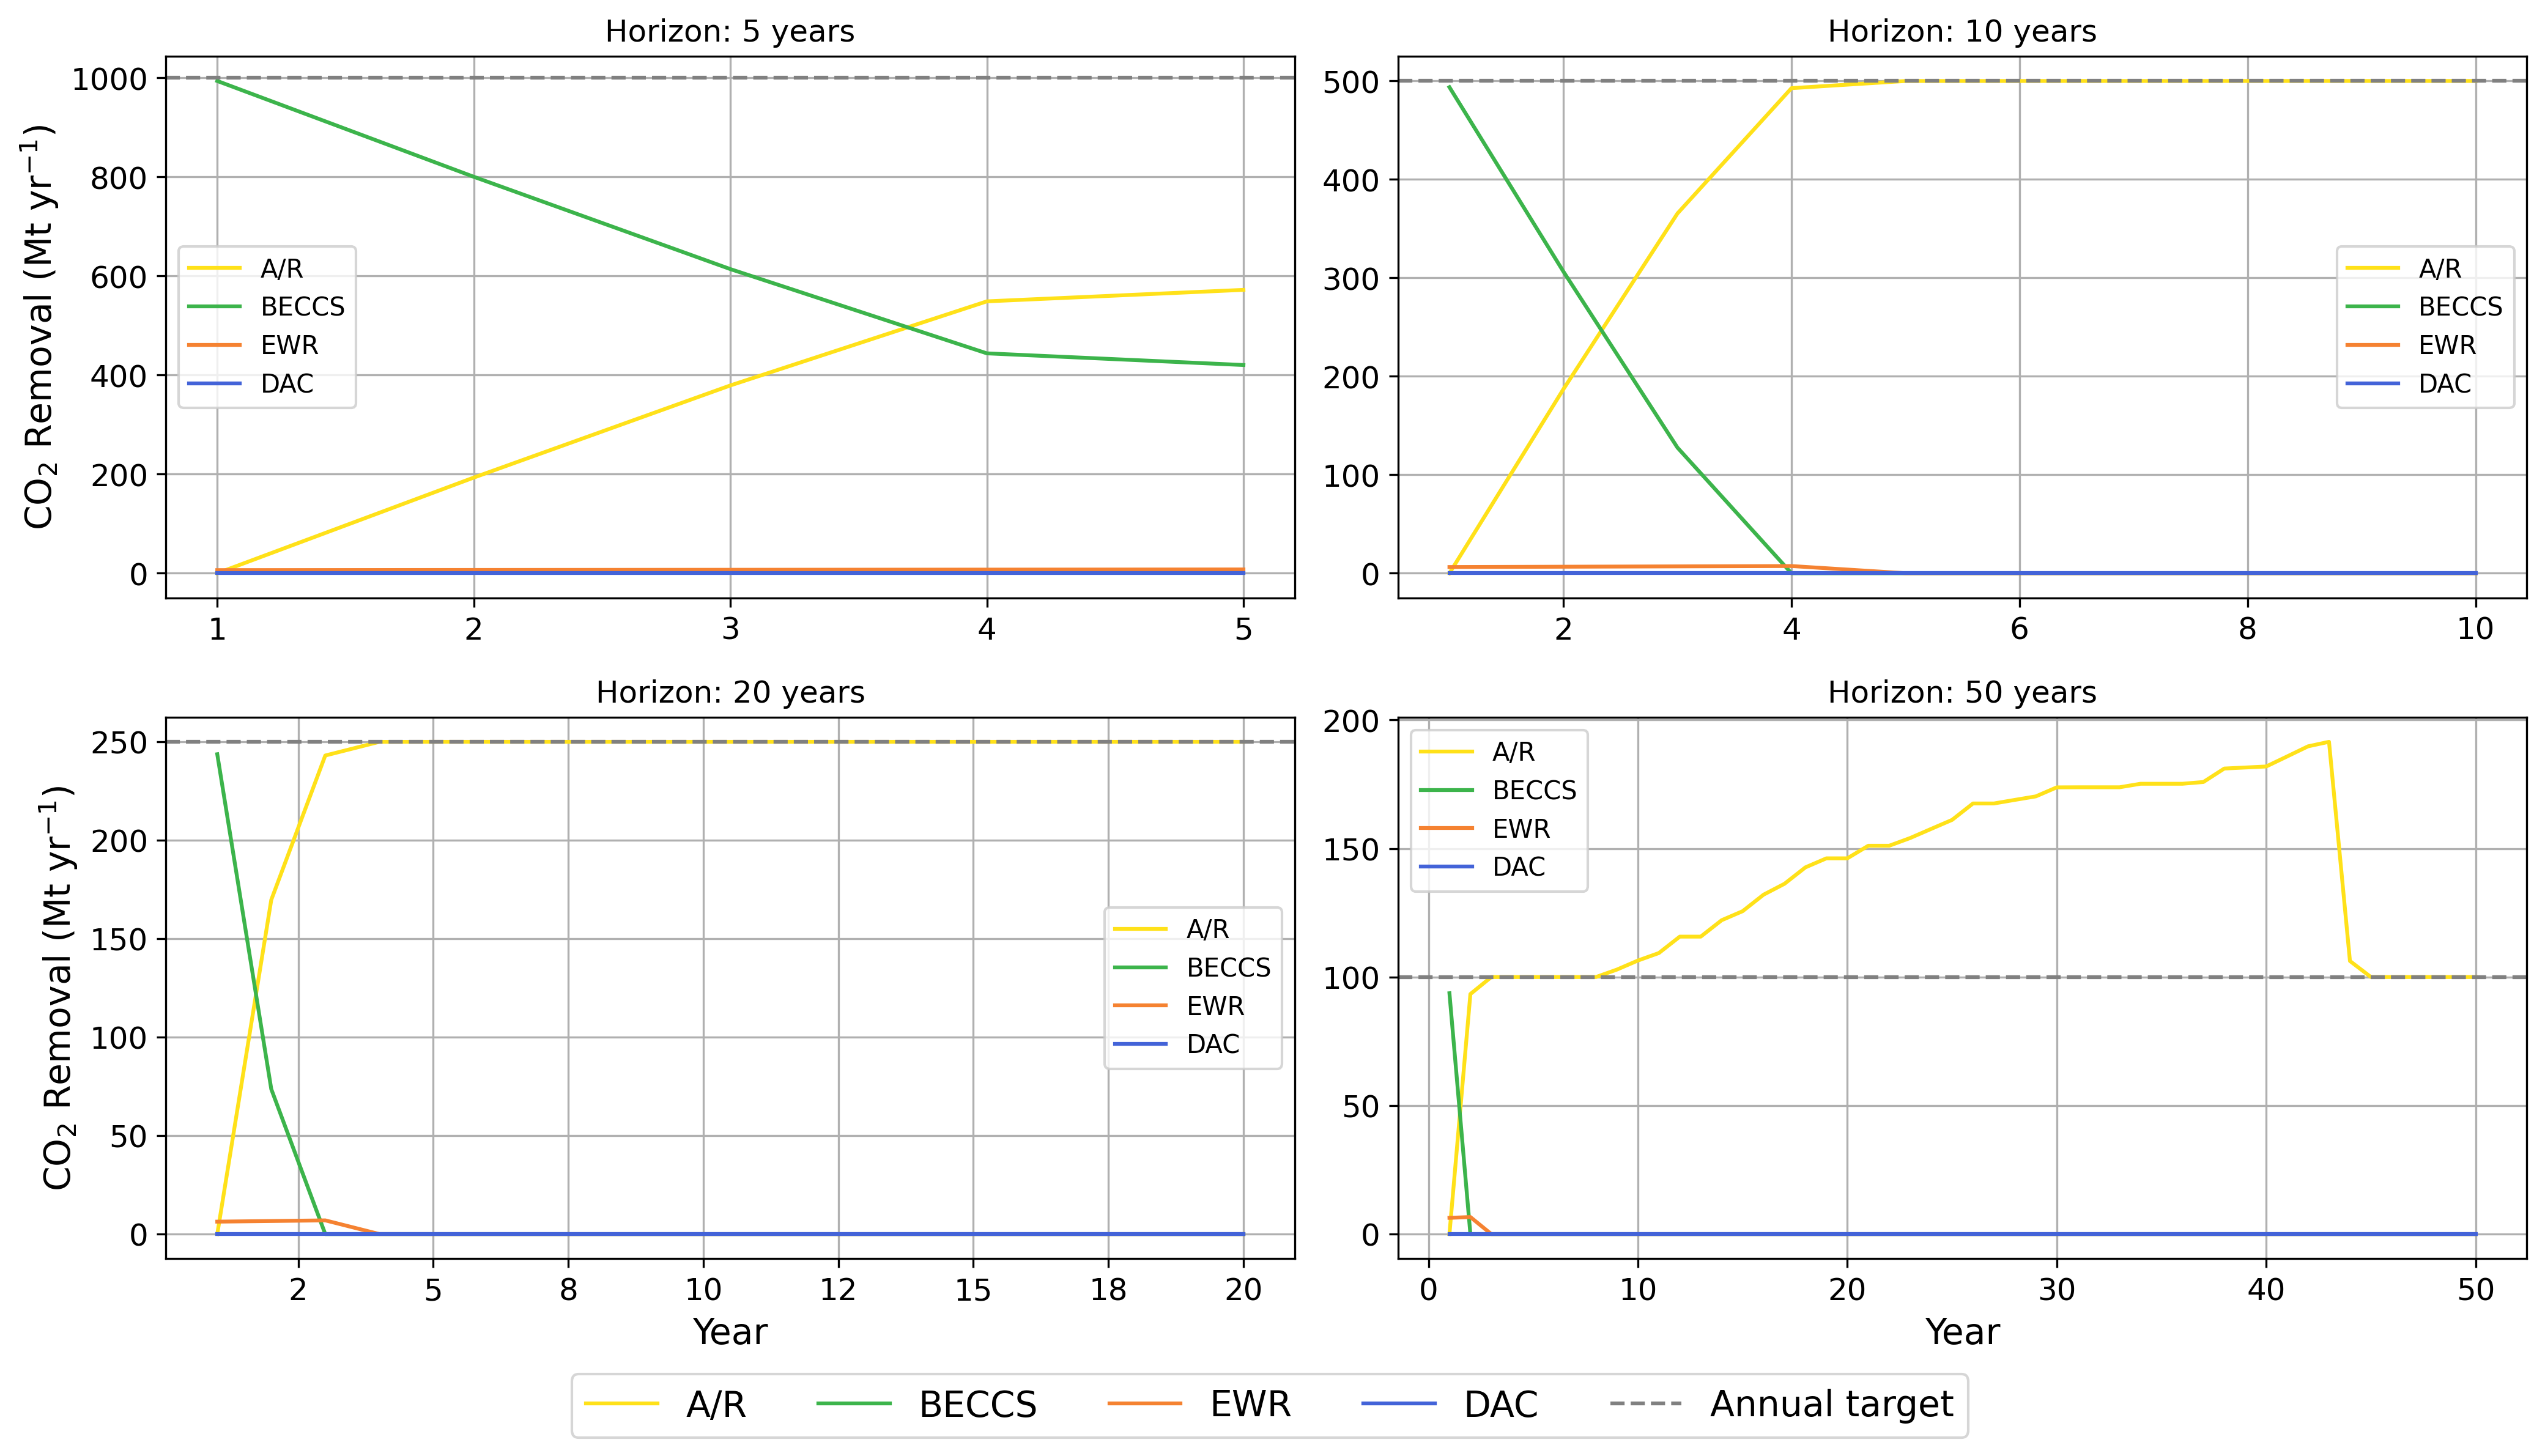
\includegraphics[width=\linewidth]{figures/annual_static_optimization_lines.png}
    \caption{Optimal static portfolio -- annual constraint}
    \label{fig:overall_static_optimization_lines}
    \vspace*{-\baselineskip}
  \end{center}
\end{figure}

\begin{table}[h!]
\renewcommand{\arraystretch}{1.4}
\adjustbox{max width=\textwidth}{%
\begin{tabular}{llrrr}
\hline
\textbf{Horizon}          & \textbf{Technology} & \textbf{Total CDR (MtCO$_2$)} & \textbf{Total Cost (M USD)} & \textbf{Average LCOC (USD)} \\ \hline
\multirow{3}{*}{5 years}  & A/R       & 1{,}899.0                   & 112{,}344  & 59.16                       \\
                          & ERW                 & 34.9                        & 890        & 25.52                       \\
                          & BECCS               & 3{,}066.1                   & 447{,}523  & 145.96                      \\ \hline
\multirow{3}{*}{10 years} & A/R       & 4{,}092.6                   & 79{,}946   & 19.53                       \\ 
                            & ERW                 & 27.2                        & 694        & 25.52                       \\
                            & BECCS               & 880.2                       & 124{,}565  & 141.52                      \\ \hline
\multirow{3}{*}{20 years} & A/R       & 4{,}680.9                   & 37{,}319   & 7.97                        \\ 
                          & ERW                 & 19.7                        & 503        & 25.52                       \\
                          & BECCS               & 299.4                       & 41{,}608   & 138.98                      \\ \hline
\multirow{3}{*}{50 years} & A/R       & 6{,}740.7                   & 24{,}432   & 3.62                        \\ 
                          & ERW                 & 12.9                        & 330       & 25.52                       \\
                        & BECCS               & 93.7                        & 12{,}656   & 135.09                      \\ \hline
\end{tabular}}
\caption{Cost and deployment by CDR technology across time horizons -- annual constraint}
\end{table}

\clearpage
\section{Alternative Dynamic Portfolio Scenarios}
\subsection{Afforestation Excluded}
In order to consider common doubts about the permanence of A/R and its comparability to other permanent NETs, this scenario excludes the use of A/R entirely. Figure A.6 presents the resulting NET portfolio. \vspace{2mm}

\begin{figure}[h!]
  \begin{center}
    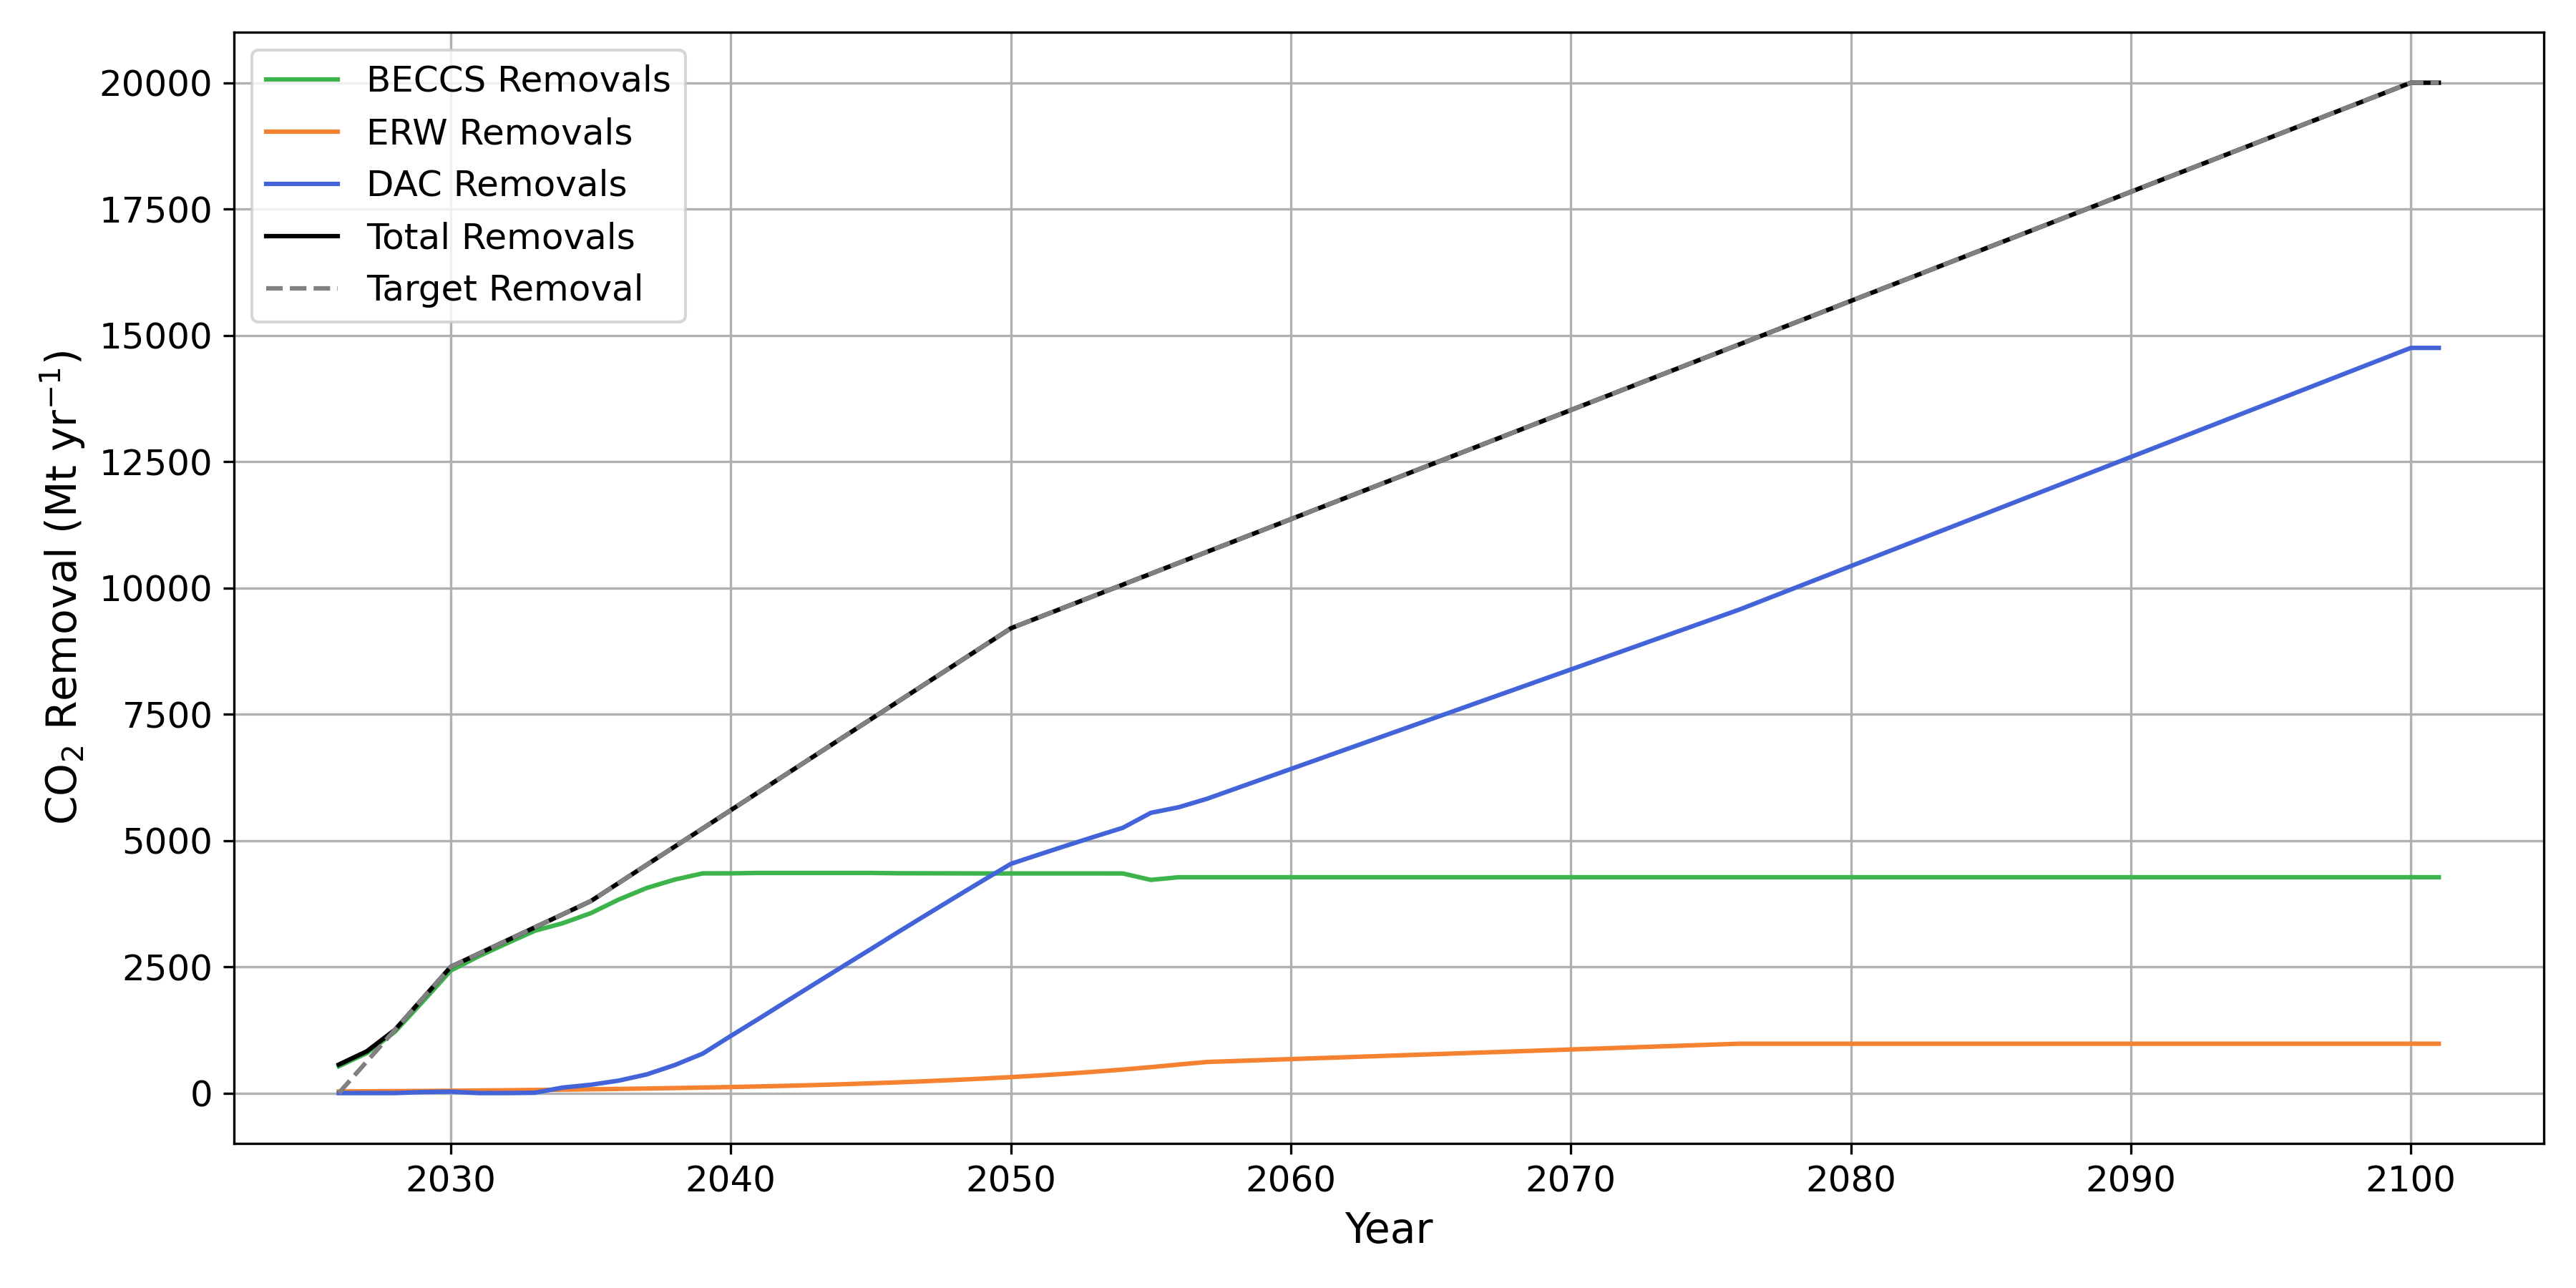
\includegraphics[width=1\linewidth]{figures/optimal_dynamic_portfolio_no_ar.png}
    \caption{Optimal dynamic portfolio with afforestation excluded}
    \label{fig:optimal_dynamic_portfolio_moreerw}
  \end{center}
  \vspace*{-\baselineskip}
\end{figure}

Compared to the baseline model, BECCS now has to fully shoulder the entire CDR demand in the early years, while large-scale DAC operations begin about 6 years earlier, in the mid-2030s. Ultimately, DAC ends up delivering a total of 528 Gt of CDR, nearly 90 Gt more than in the baseline portfolio. The overall contribution of BECCS is increased by about 17 Gt, caused by the earlier ramp-up, while the ERW pathway remains unchanged. Looking at the cost of this scenario, the total cost has increased by 15\% to a total of about 204 trillion USD, with the average cost increasing from 201.71 USD to 232.43 USD tCO$_2^{-1}$. This significant increase demonstrates that including afforestation in CDR portfolios to delivery cheap, early results is an essential lever to improve the overall economic viability of large-scale carbon removal.

\begin{table}[h!]
\adjustbox{max width=\textwidth}{%
\renewcommand{\arraystretch}{1.4}
\begin{tabular}{lrrr}
\hline
\textbf{Technology} & \textbf{Amount removed (Mt)} & \textbf{Total cost (B USD)} & \textbf{Average cost (USD)} \\ \hline

\textbf{ERW}   & 46{,}154.01  & 1{,}284.19  & 27.82 \\
\textbf{BECCS} & 305{,}083.90 & 54{,}594.50 & 178.95 \\
\textbf{DAC}   & 527{,}777.62 & 148{,}159.60 & 280.72 \\ \hline

\textbf{Total} & 879{,}015.53  & 204{,}038.29 & 232.12 \\ \hline
\end{tabular}}
\caption{Breakdown of amounts removed and cost by NET - no afforestation}
\end{table}

\subsection{Afforestation using Forest Plantations}
The baseline portfolio presented in chapter 4 uses assisted natural regeneration for afforestation. Figure A.7 presents an alternative scenario which uses forest plantations, that is manually planted forests, instead.\vspace{2mm}

\begin{figure}[h!]
  \begin{center}
    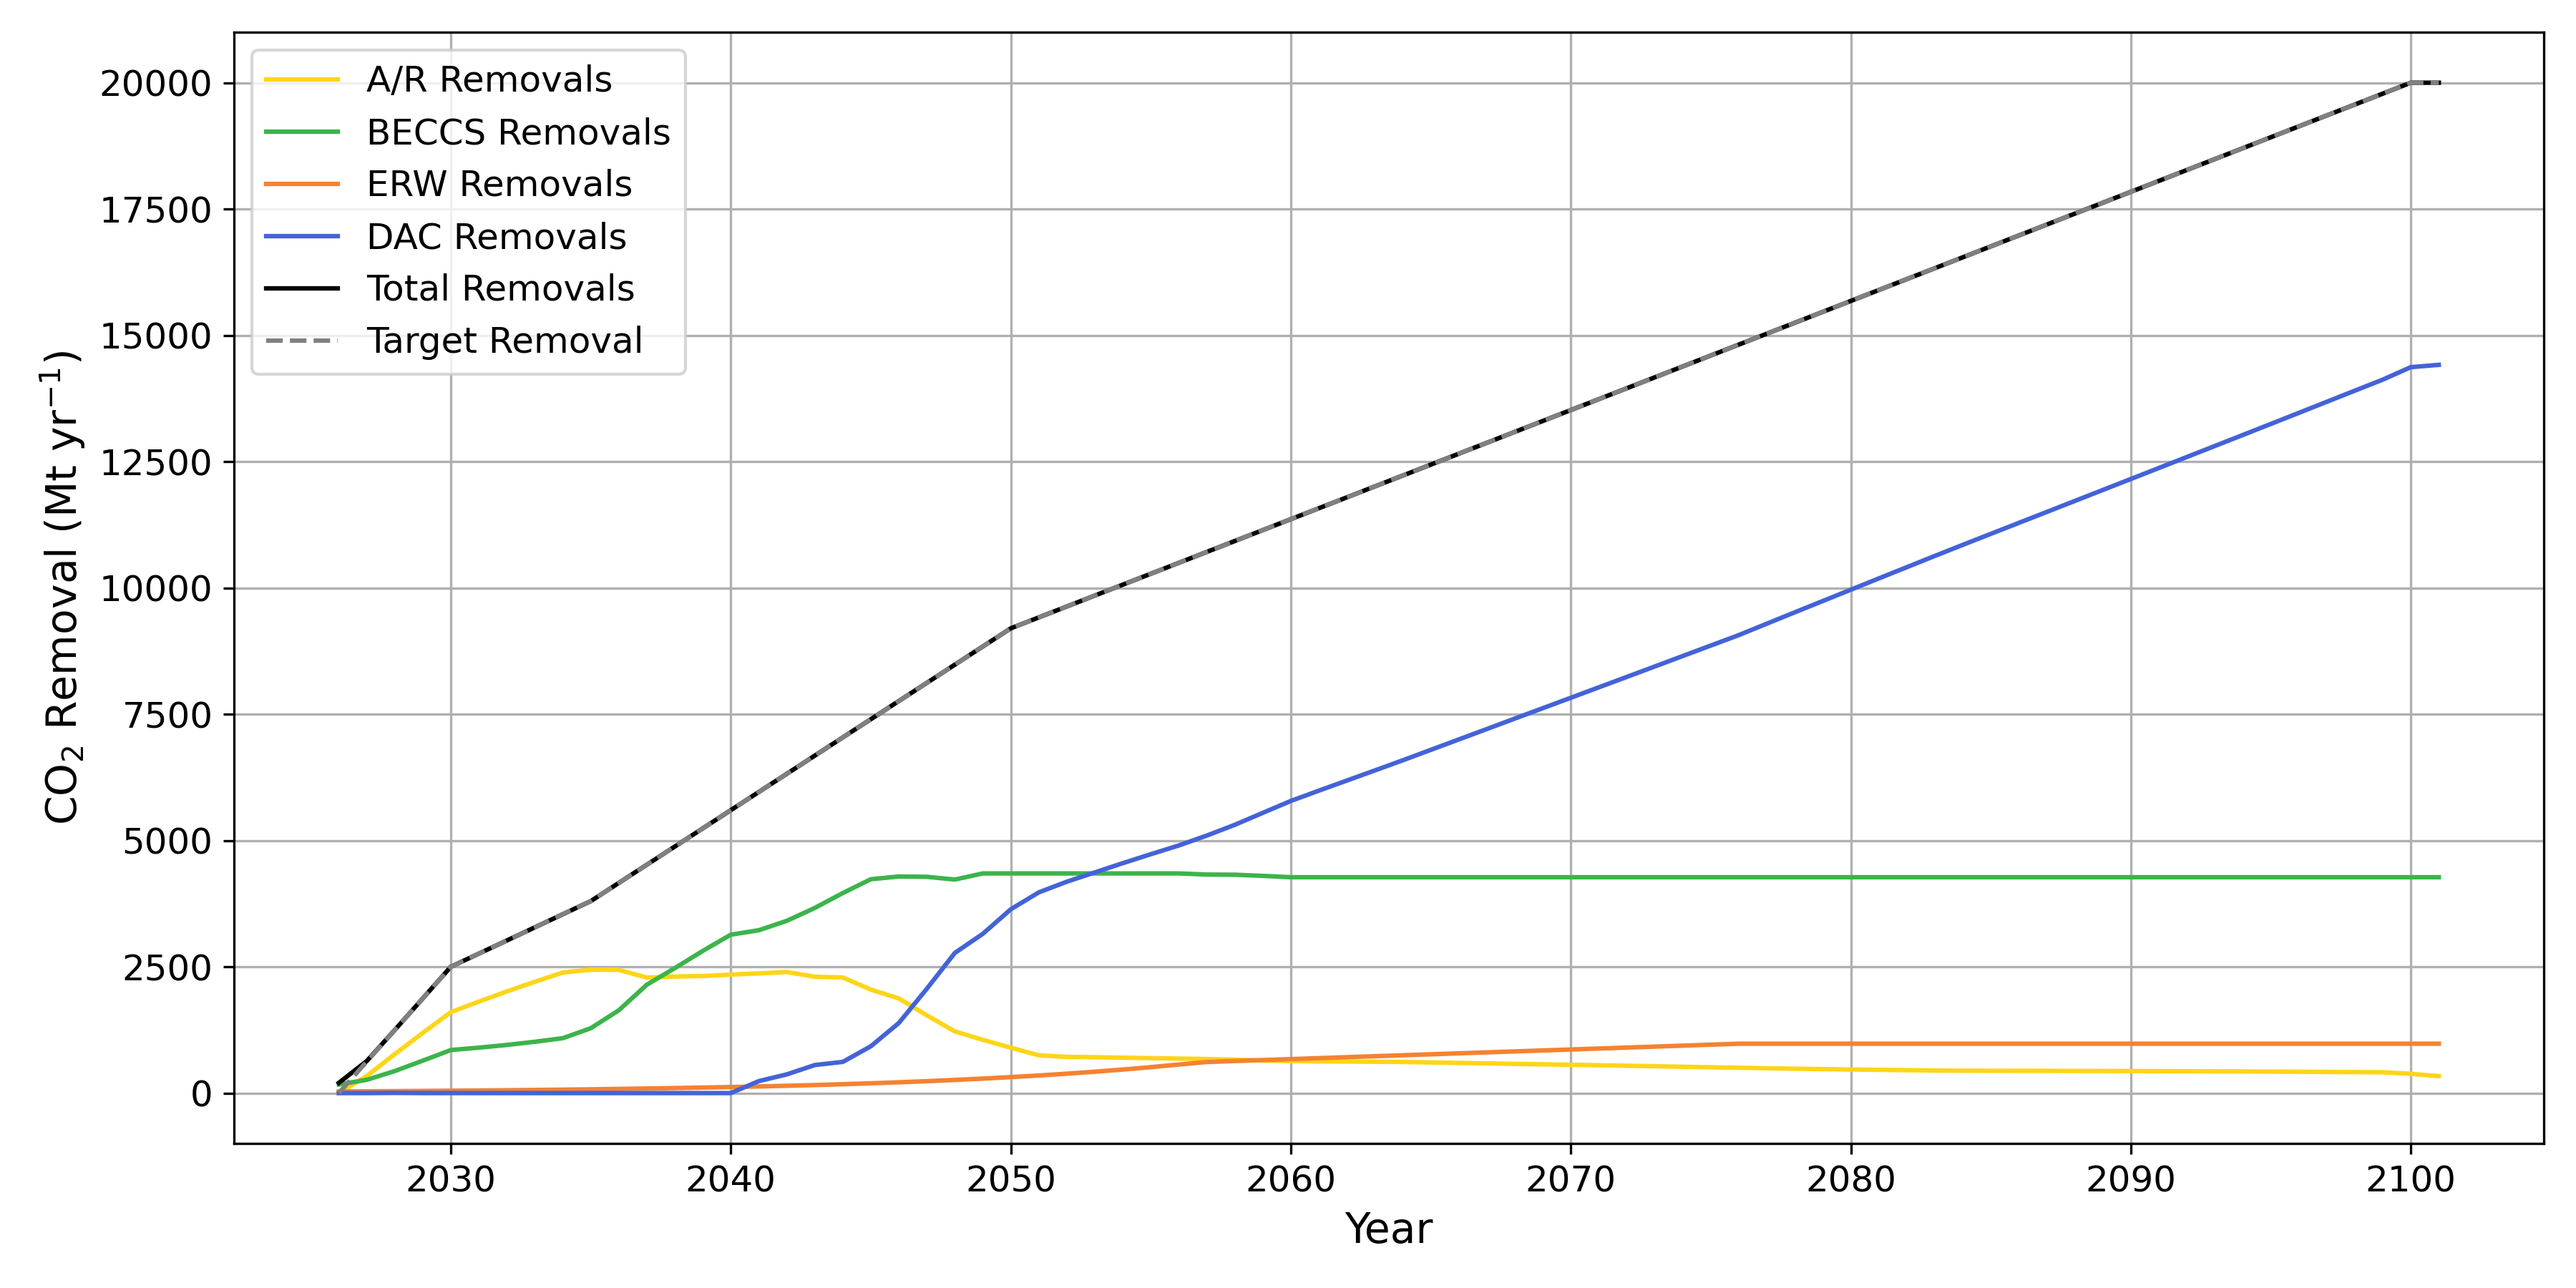
\includegraphics[width=1\linewidth]{figures/optimal_dynamic_portfolio_planted_ar.png}
    \caption{Optimal dynamic portfolio using forest plantation}
    \label{fig:optimal_dynamic_portfolio_planted_ar}
  \end{center}
  \vspace*{-\baselineskip}
\end{figure}

Compared to the baseline model, A/R ramps up faster, but also shows exhaustion much earlier, with the decline beginning already in the 2040s. Considering the much faster but shorter growth cycles of forest plantations (see Figure 3.3), this is the expected result. Looking at the amount removed by A/R and the respective LCOC, this scenario shows a significantly lower overall contribution of A/R at 71 GtCO$_2$, compared to 106 Gt in the baseline scenario, and a much higher LCOC of 68.99 USD tCO$_2^{-1}$. This matches the MACC presented in Figure 3.5, and shows that while using forest plantations may initially deliver faster CDR, its overall effect is negative in regards to both, the A/R potential and the associated costs.

\begin{table}[h!]
\adjustbox{max width=\textwidth}{%
\renewcommand{\arraystretch}{1.4}
\begin{tabular}{lrrr}
\hline
\textbf{Technology} & \textbf{Amount removed (Mt)} & \textbf{Total cost (B USD)} & \textbf{Average cost (USD)} \\ \hline

\textbf{A/R}   & 71{,}312.62  & 4{,}920.13  & 68.99 \\
\textbf{ERW}   & 46{,}154.01  & 1{,}284.19  & 27.82 \\
\textbf{BECCS} & 278{,}267.96 & 49{,}438.34 & 177.66 \\
\textbf{DAC}   & 482{,}726.66 & 135{,}647.66 & 281.00 \\ \hline

\textbf{Total} & 878{,}461.25 & 191{,}290.32 & 217.76 \\ \hline
\end{tabular}}
\caption{Breakdown of amounts removed and cost by NET - forest plantation}
\end{table}

\subsection{Increased Enhanced Weathering}
Figure A.8 presents another alternative scenario, in which which the the available rock material was doubled to start at 1\% of the global coal mining capacity and increase to 30\% over 50 years, while the annual allowable increase compared to the previous year was also doubled to 20\%.\vspace{2mm}

\begin{figure}[h!]
  \begin{center}
    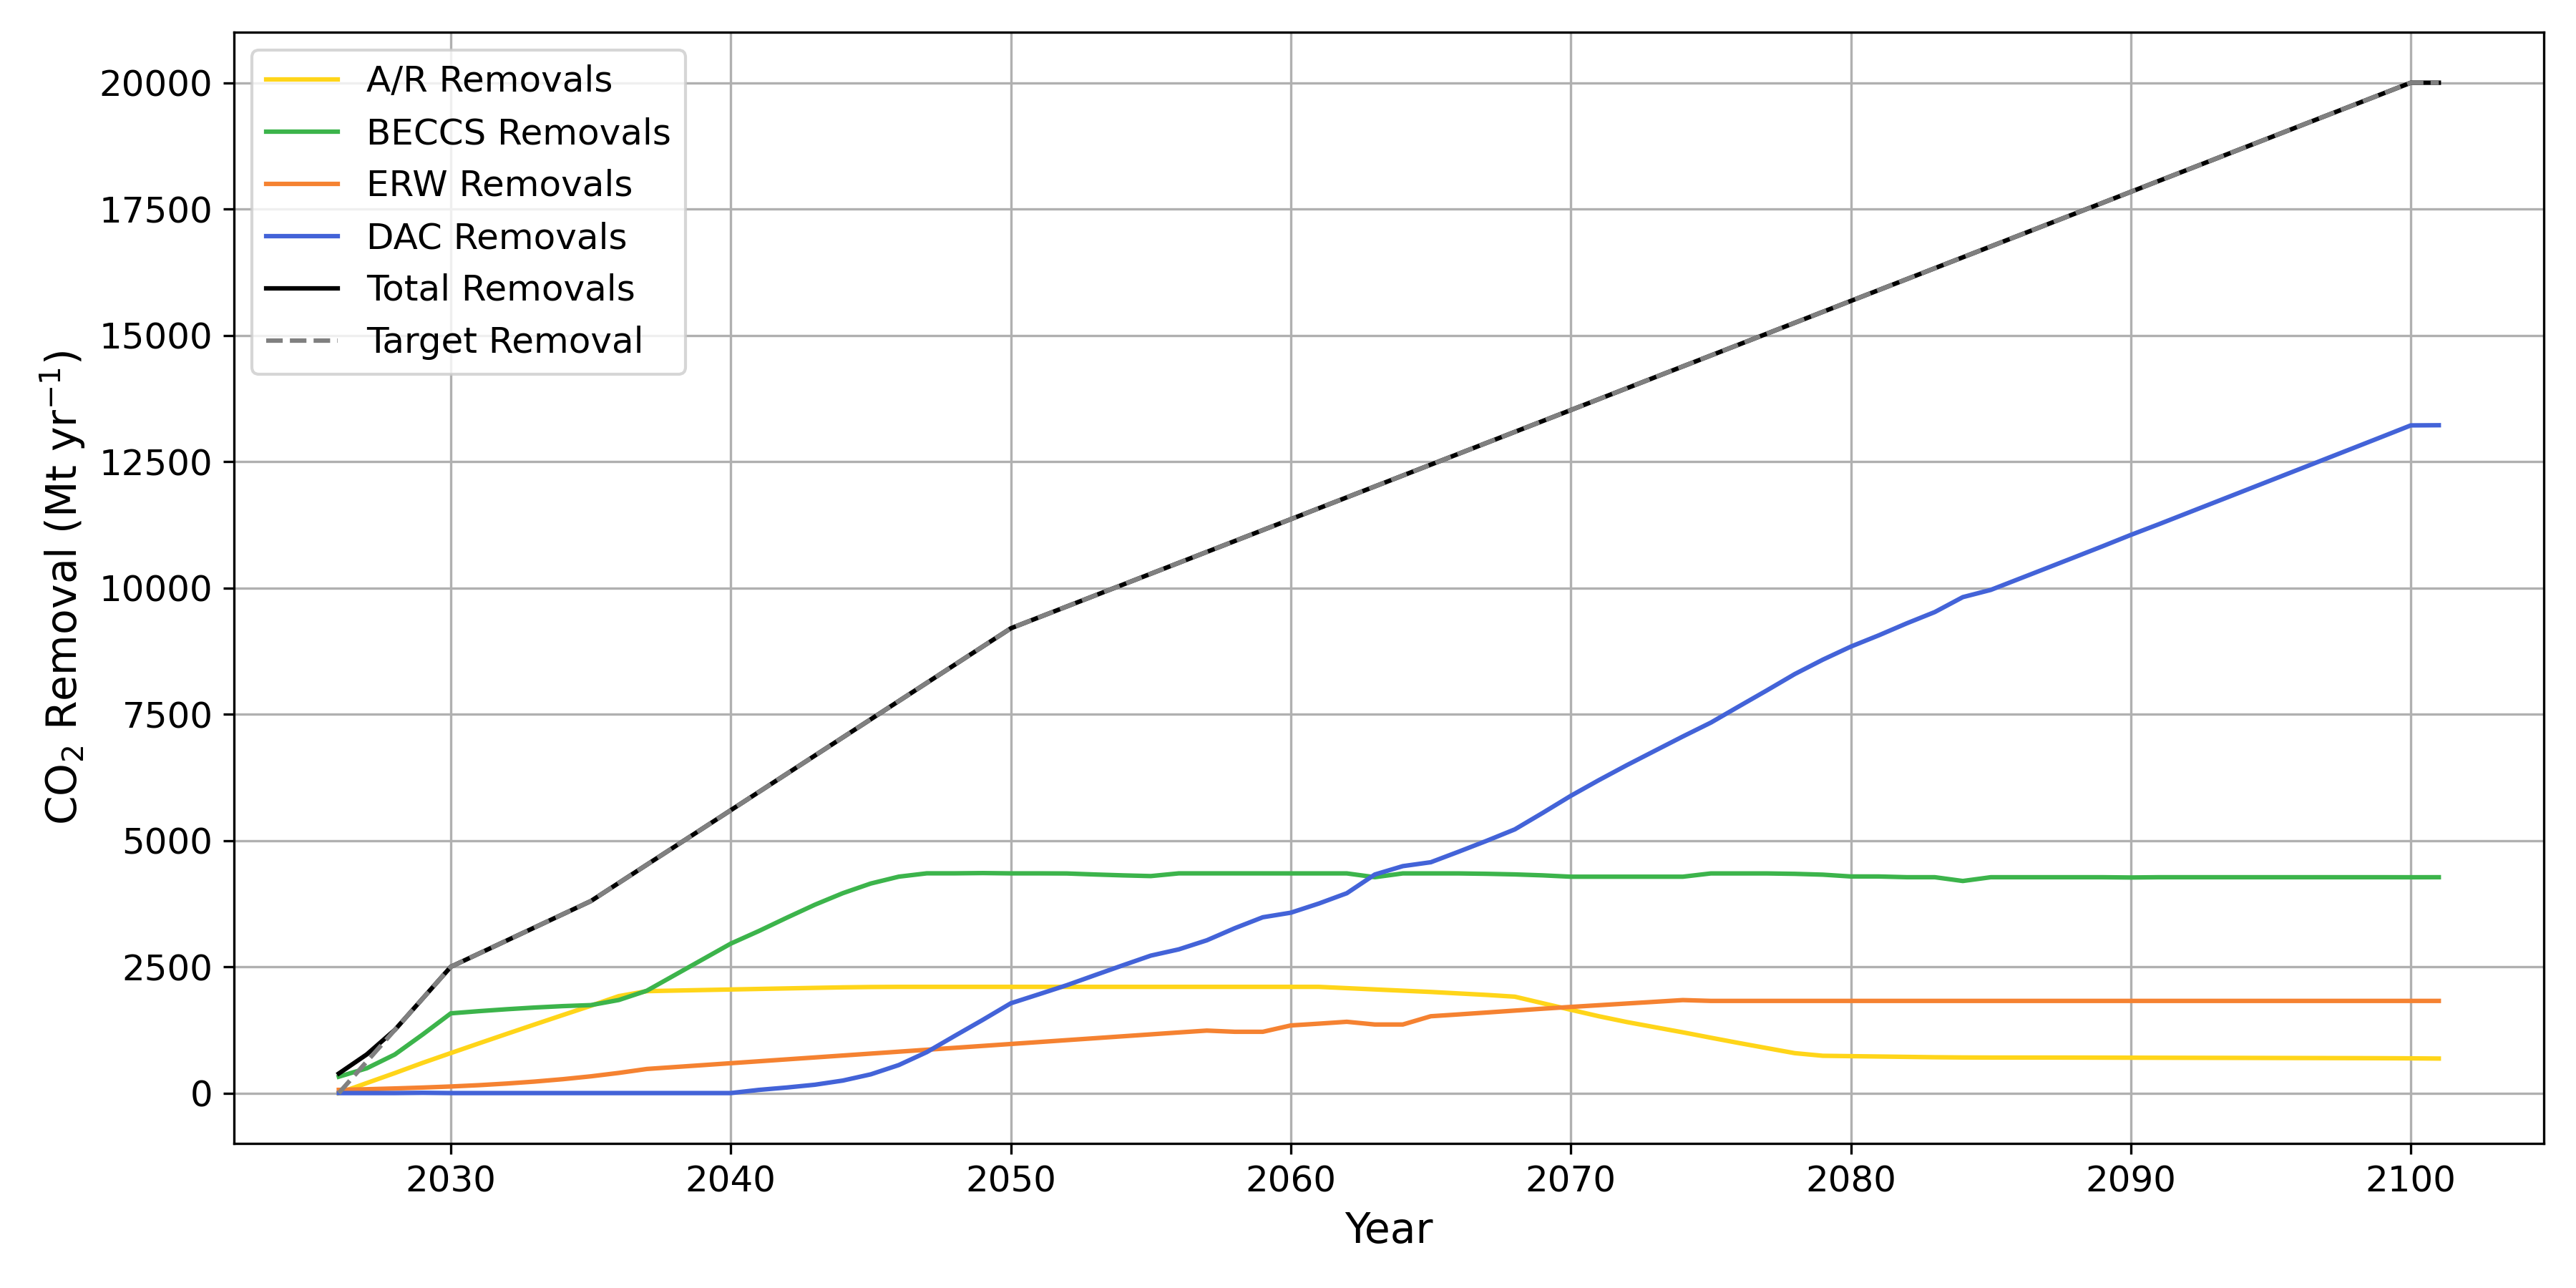
\includegraphics[width=1\linewidth]{figures/optimal_dynamic_portfolio_more_erw.png}
    \caption{Optimal dynamic portfolio with increased ERW}
    \label{fig:optimal_dynamic_portfolio_moreerw}
  \end{center}
  \vspace*{-\baselineskip}
\end{figure}

Comparing the results to the baseline model, ERW, as expected, takes a much larger share of the overall portfolio and ends up delivering about 2.3 Gt of CDR annually and over 95 Gt overall by 2100, compared to 46 Gt in the base model. This increase is balanced out by delay of DAC operations by a few years, and a reduction its contributions from 439 GtCO$_2$ in the base model to 394 Gt, while the deployment profiles of A/R and BECCS remain largely stable. Overall, the deployment timeline does not materially change, showing that the recommendations regarding investments and policies derived from the base model remain true even if ERW is ramped up more quickly than expected. Looking at the overall costs, we see a reduction in the weighted average cost from 201.71 USD to only 188.53 USD tCO$_2^{-1}$ due to the increase in lower-cost CDR from ERW.

\begin{table}[h!]
\adjustbox{max width=\textwidth}{%
\renewcommand{\arraystretch}{1.4}
\begin{tabular}{lrrr}
\hline
\textbf{Technology} & \textbf{Amount removed (Mt)} & \textbf{Total cost (B USD)} & \textbf{Average cost (USD)} \\ \hline

\textbf{A/R}   & 105{,}629.34 & 1{,}085.26  & 10.27 \\
\textbf{ERW}   & 95{,}405.32  & 2{,}717.61  & 28.48 \\
\textbf{BECCS} & 284{,}193.00 & 50{,}500.17 & 177.70 \\
\textbf{DAC}   & 393{,}550.33 & 111{,}246.92 & 282.68 \\ \hline

\textbf{Total} & 878{,}777.99 & 165{,}549.96 & 188.39 \\ \hline
\end{tabular}}
\caption{Breakdown of amounts removed and cost by NET - increased ERW}
\end{table}